% per_layer_curvature.tex
% ACM sigconf 风格中文论文：三层 RQ-VAE 的逐层可学习双曲曲率
% 编译: xelatex per_layer_curvature.tex (需 ctex / xeCJK)

\documentclass[sigconf, nonacm, anonymize, 9pt]{acmart}

% 中文支持：使用 ctex (xelatex)
\usepackage{ctex}
\usepackage{amsmath, amssymb}
\usepackage{booktabs}
\usepackage{graphicx}
\usepackage{hyperref}
\usepackage{multirow}
\usepackage{tikz}
\usetikzlibrary{arrows.meta, positioning}

% acmart 与 ctex 行距冲突修复：恢复 \baselinestretch 原值，
% 避免 AtEndDocument 报错中断参考文献页输出
\makeatletter
\let\baselinestretch\ACM@origbaselinestretch
\makeatother

% 段落溢出缓解（\leq 5pt 的微超栏）
\emergencystretch=1.5em

% 段落顶格（无首行缩进），以段间距分隔
\setlength{\parindent}{0pt}
\setlength{\parskip}{2pt}

% 常用数学算子
\DeclareMathOperator{\arctanh}{arctanh}
\DeclareMathOperator{\argmin}{arg\,min}
\DeclareMathOperator{\argmax}{arg\,max}

% ====== 元数据 ======
\title{Per-Layer Learnable Hyperbolic Curvature for Three-Layer RQ-VAE in Generative Recommendation}
\renewcommand{\shorttitle}{Per-Layer Learnable Curvature for Three-Layer RQ-VAE}

\author{Anonymous}
\renewcommand{\shortauthors}{Anonymous}

\begin{document}

\maketitle

% ===========================================================
% 1 引言
% ===========================================================
\section{引言}

\subsection{分层码本的几何异质性与共享曲率的局限}

RQ-VAE~\cite{lee2022rqvae} 通过逐层量化残差，将连续 item representation 转换为 coarse-to-fine 的离散 semantic identifiers~\cite{rajput2023tiger,singh2024rqvae}。给定编码表示 $z$，第 $\ell$ 层从码本
\begin{equation}
\mathcal{E}_{\ell}=\{e_{\ell k}\}_{k=1}^{K_{\ell}}
\end{equation}
中选择与当前残差最接近的码字，并将尚未被解释的信息传递至下一层：
\begin{equation}
r_0=z,\qquad
k_\ell^{*}=\argmin_k d(r_\ell,e_{\ell k}),\qquad
r_{\ell+1}=r_\ell-e_{\ell k_\ell^{*}}.
\end{equation}
因此，不同 RQ stage 实际处理的是逐层变化的 residual representation。本文关注的问题是：\emph{当不同量化层形成不同的表示结构时，是否仍应要求它们共享完全相同的几何度量和曲率？}

semantic tokenization 不仅需要压缩 item embeddings，还需要保留对推荐有用的 item relationships——仅依赖 reconstruction 的 RQ-VAE 可能破坏 item neighborhood，而显式保留 topology 可得到更有效的 semantic tokens（CoST~\cite{jin2024cost}、TopoTok~\cite{topotok2026}）。据此，我们依次验证两个问题：
\noindent(1)\ 不同 RQ stage 是否形成了相同的 codebook geometry？\\[2pt]
\noindent(2)\ 若不同，各层是否具有不同的 curvature preference？

\noindent\textbf{问题 1：codebook geometry 是否层间一致？}

\noindent\textbf{观察 1（residual 异质性）。} 在 Vanilla-RQ 中：

\noindent\textbullet\ 三层 residual norm 均值随量化深度稳定下降，Kolmogorov\-Smirnov 检验表明各 stage 分布显著不同。\\[2pt]
\noindent\textbullet\ 在统一码本规模
\begin{equation}
K\in\{64,128,256\},
\end{equation}
下，layer-dependent pattern 保持稳定，说明该异质性是 residual quantization 深化本身的结构性结果。

\noindent\textbf{观察 2（codebook 几何异质性）。} 三个层面的指标（表~\ref{tab:equal-k-pairwise}、图~\ref{fig:codebook-geometry}）呈现逐层一致的模式：

\noindent\textbullet\ \emph{全局}：$\bar d_{\mathrm{pair}}^{(0)}>\bar d_{\mathrm{pair}}^{(1)}>\bar d_{\mathrm{pair}}^{(2)}$，L0/L2 码字间距比 $2.25\times$--$2.49\times$；\\[2pt]
\noindent\textbullet\ \emph{局部}：NN distance 逐层递减（L0/L2 比 $1.60\times$--$1.78\times$），local density 递增；\\[2pt]
\noindent\textbullet\ \emph{谱}：effective rank 递增而第一主方向方差递减——排除``同一结构的均匀缩放''这一替代解释。

\begin{table}[ht]
\centering
\small
\caption{三层 codebook 几何异质性汇总（三种统一码本规模 $K=64/128/256$）。KS/$W_1$ 为 $K=128$ 下 L0 与 L2 完整 pairwise-distance distributions 的差异；NN ratio 为 L0/L2 平均 nearest-neighbor distance 之比。}
\label{tab:equal-k-pairwise}
\begin{tabular}{lccc}
\toprule
Metric & L0 & L1 & L2 \\
\midrule
\multicolumn{4}{l}{\textit{Mean pairwise distance}} \\
$K=64$  & 0.1922 & 0.1059 & 0.0856 \\
$K=128$ & 0.1946 & 0.1060 & 0.0839 \\
$K=256$ & 0.1993 & 0.1035 & 0.0799 \\
\midrule
\multicolumn{4}{l}{\textit{NN distance}} \\
$K=64$  & 0.1095 & 0.0809 & 0.0686 \\
$K=128$ & 0.1044 & 0.0767 & 0.0641 \\
$K=256$ & 0.1015 & 0.0703 & 0.0570 \\
\midrule
\multicolumn{4}{l}{\textit{Local density ($k=5$)}} \\
$K=64$  & 8.08 & 11.78 & 13.97 \\
$K=128$ & 8.47 & 12.46 & 14.96 \\
$K=256$ & 8.89 & 13.52 & 16.74 \\
\midrule
\multicolumn{4}{l}{\textit{Effective rank}} \\
$K=64$  & 12.80 & 18.54 & 20.05 \\
$K=128$ & 15.65 & 22.17 & 23.64 \\
$K=256$ & 17.61 & 24.31 & 25.77 \\
\midrule
\multicolumn{4}{l}{\textit{PC1 variance}} \\
$K=64$  & $21.89\%$ & $8.92\%$ & $7.76\%$ \\
$K=128$ & $20.54\%$ & $8.36\%$ & $6.33\%$ \\
$K=256$ & $17.52\%$ & $7.20\%$ & $5.58\%$ \\
\midrule
NN ratio (L0/L2) & \multicolumn{3}{l}{$1.60\times$ / $1.63\times$ / $1.78\times$\ ($K=64/128/256$)} \\
KS / $W_1$ (L0 vs.\ L2, $K=128$) & \multicolumn{3}{l}{$D_{\mathrm{KS}}=0.9824$,\quad $W_1=0.1107$} \\
\bottomrule
\end{tabular}
\end{table}

\begin{figure*}[t]
\centering
\Description{三层码本几何异质性的三面板定量证据：全局尺度、局部结构与谱形状。}
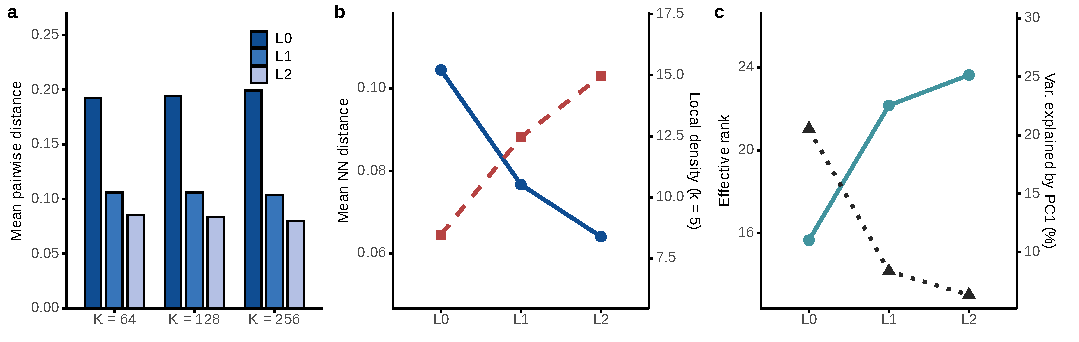
\includegraphics[width=\textwidth]{figures/codebook_geometry_3panel.pdf}
\caption{三层 codebook 几何异质性。\textbf{a}，不同统一码本规模下平均 pairwise distance（对应表~\ref{tab:equal-k-pairwise}）；\textbf{b}，$K=128$ 时平均 nearest-neighbor distance 与 local density；\textbf{c}，$K=128$ 时 effective rank 与第一主方向方差占比。随着 RQ depth 增加，码本几何由 broad/sparse/anisotropic 向 compact/dense/more isotropic 过渡。}
\label{fig:codebook-geometry}
\end{figure*}

因此，随 RQ depth 增加，codebook geometry 由
\begin{equation}
\text{broad / sparse / anisotropic}\ \longrightarrow\ \text{compact / dense / more isotropic},
\end{equation}
过渡，可概括为
\begin{equation}
G(\mathcal{E}_0)\neq G(\mathcal{E}_1)\neq G(\mathcal{E}_2),
\end{equation}
其中 $G(\mathcal{E}_\ell)$ 表示由全局距离、局部邻域与谱结构共同描述的第 $\ell$ 层 codebook geometry。

\noindent\textbf{从几何异质到曲率异质。} codebook geometry 不同本身不足以推出 curvature 不同：(i) 距离尺度的差异可由全局缩放解释；(ii) RQ-VAE 的输入是连续 item embeddings 而非 graph，不能依预设 tree/graph 假设推断双曲。

\noindent\textbf{问题 2：各层是否具有不同的 curvature preference？}

\noindent\textbf{诊断方法（图~\ref{fig:curvature-diagnostic}）。} 构造 curvature-independent relational reference：对每个 codeword，由其量化 items 与其他 codeword 对应 items 的关系构造 item-induced affinity，保留 top-10 邻接形成 relational graph，以图上 shortest-path distance 定义参考距离
\begin{equation}
D_\ell^{\mathrm{ref}}.
\end{equation}
$D_\ell^{\mathrm{ref}}$ 并非 ground-truth geometry，仅回答：\emph{哪一种曲率能以更低失真表达已学习到的 item 关系？}（与 topology-preserving tokenization 动机一致~\cite{jin2024cost,topotok2026}）

\begin{figure}[ht]
\centering
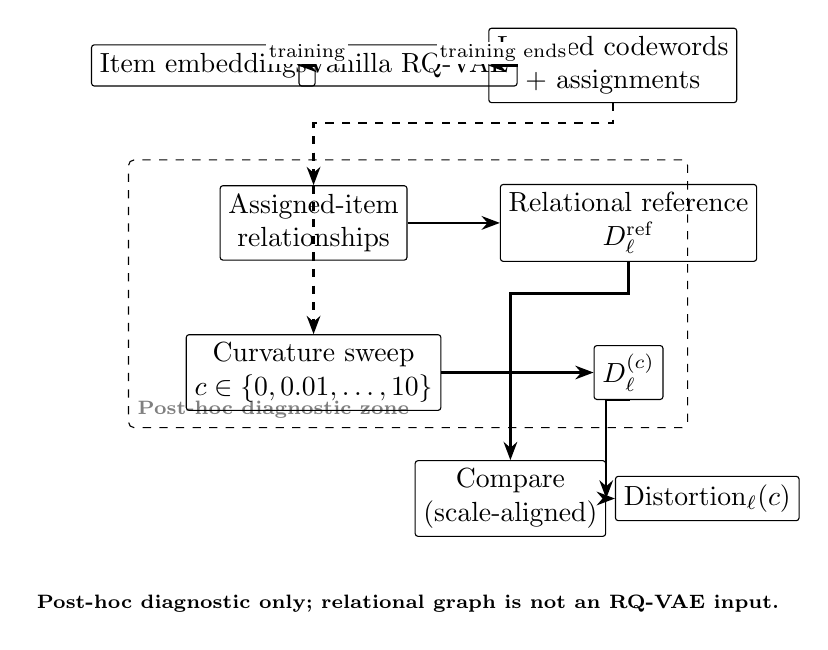
\begin{tikzpicture}[
  box/.style={draw, rounded corners=1pt, align=center, inner sep=3pt, font=\normalsize},
  dbox/.style={draw, dashed, rounded corners=2pt, align=center, inner sep=4pt},
  arrow/.style={-{Stealth}, thick},
  darrow/.style={-{Stealth}, thick, dashed},
  lab/.style={font=\scriptsize, fill=white, inner sep=1pt}
]
  \node[box] (n1) at (0,0) {Item embeddings};
  \node[box] (n2) at (2.6,0) {Vanilla RQ-VAE};
  \node[box] (n3) at (5.2,0) {Learned codewords\\ + assignments};
  \draw[arrow] (n1) -- node[lab, above] {training} (n2);
  \draw[arrow] (n2) -- node[lab, above] {training ends} (n3);

  \node[dbox, minimum width=7.1cm, minimum height=3.4cm] (zone) at (2.6,-2.9) {};
  \node[font=\scriptsize, text=gray, anchor=south west] at (zone.south west) {\textbf{Post-hoc diagnostic zone}};

  \node[box] (n4) at (1.4,-2.0) {Assigned-item\\ relationships};
  \node[box] (n5) at (5.4,-2.0) {Relational reference\\ $D_\ell^{\mathrm{ref}}$};
  \node[box] (n6) at (1.4,-3.9) {Curvature sweep\\ $c\in\{0,0.01,\dots,10\}$};
  \node[box] (n7) at (5.4,-3.9) {$D_\ell^{(c)}$};
  \draw[darrow] (n3.south) -- ++(0,-0.25) -| (n4.north);
  \draw[darrow] (n3.south) -- ++(0,-0.25) -| (n6.north);
  \draw[arrow] (n4) -- (n5);
  \draw[arrow] (n6) -- (n7);

  \node[box] (n8) at (3.9,-5.5) {Compare\\ (scale-aligned)};
  \node[box] (n9) at (6.4,-5.5) {$\mathrm{Distortion}_\ell(c)$};
  \draw[arrow] (n7) -- ++(0,-0.35) -| (n8.east);
  \draw[arrow] (n5.south) -- ++(0,-0.4) -| (n8.north);
  \draw[arrow] (n8) -- (n9);

  \node[font=\scriptsize, align=center, anchor=north] at (2.6,-6.6)
    {\textbf{Post-hoc diagnostic only; relational graph is not an RQ-VAE input.}};
\end{tikzpicture}
\caption{Post-hoc curvature preference diagnostic。训练结束后，从 codewords 与 assignments 出发：由 assigned-item relationships 构造 relational reference $D_\ell^{\mathrm{ref}}$，对同一 codewords 在 $c\in\{0,0.01,\dots,10\}$ 上计算 $D_\ell^{(c)}$，经全局尺度对齐后比较 distortion。relational graph 仅用于训练后诊断，不是 RQ-VAE 的输入。}
\label{fig:curvature-diagnostic}
\end{figure}



随后在曲率集合
\begin{equation}
c\in\{0,0.01,0.05,0.1,0.5,1,2,5,10\}
\end{equation}
上 sweep（$c=0$ 即 Euclidean geometry），对每个 layer--curvature pair 求解最优全局尺度
\begin{equation}
a_{\ell,c}^{*}=\argmin_a \sum_{i,j}\left(aD_\ell^{(c)}(i,j)-D_\ell^{\mathrm{ref}}(i,j)\right)^2.
\end{equation}
并计算归一化 distortion
\begin{equation}
\mathrm{Distortion}_{\ell}(c)=\frac{\sum_{i,j}\left(a_{\ell,c}^{*}D_\ell^{(c)}(i,j)-D_\ell^{\mathrm{ref}}(i,j)\right)^2}{\sum_{i,j}\left(D_\ell^{\mathrm{ref}}(i,j)\right)^2}.
\end{equation}
\noindent\textbf{结果（图~\ref{fig:curvature-distortion}、表~\ref{tab:curvature-summary}、表~\ref{tab:curvature-robustness}）。}
\noindent\textbullet\ L0 的最低 distortion 出现在 $c^{*}=0$（Euclidean preference）；\\[2pt]
\noindent\textbullet\ L1/L2 的最低点位于 $c^{*}\geq 1$（hyperbolic preference），相比 Euclidean 改善 $1.4\%$/$1.3\%$；\\[2pt]
\noindent\textbullet\ 该 ordering 在 $K=64/128/256$ 下完全稳定，且不因全局尺度 $a_{\ell,c}^{*}$ 的优化而消失；Spearman correlation、kNN overlap 与 Gromov $\delta$-hyperbolicity~\cite{gromov1987hyperbolic} 辅助分析一致。

\begin{table}[ht]
\centering
\small
\caption{$K=128$ 下各层 curvature preference 汇总。Gromov $\delta$/diam 为归一化 hyperbolicity 度量。}
\label{tab:curvature-summary}
\begin{tabular}{lccc}
\toprule
Metric & L0 & L1 & L2 \\
\midrule
Best $c^{*}$ & $0$ & $\geq 1$ & $\geq 1$ \\
Min distortion & 0.0352 & 0.0280 & 0.0297 \\
Euclidean distortion & 0.0352 & 0.0284 & 0.0301 \\
Hyp. improvement & $0\%$ & $1.4\%$ & $1.3\%$ \\
Gromov $\delta$/diam & 0.318 & 0.303 & 0.425 \\
\bottomrule
\end{tabular}
\end{table}

\begin{table}[ht]
\centering
\small
\caption{三种统一码本规模下的 best curvature ordering（robustness）。}
\label{tab:curvature-robustness}
\begin{tabular}{lccc}
\toprule
$K$ & L0 best $c^{*}$ & L1 best $c^{*}$ & L2 best $c^{*}$ \\
\midrule
$K=64$   & $0$   & $\geq 1$ & $\geq 1$ \\
$K=128$  & $0$   & $\geq 1$ & $\geq 1$ \\
$K=256$  & $0$   & $\geq 1$ & $\geq 1$ \\
\bottomrule
\end{tabular}
\end{table}

\begin{figure}[ht]
\centering
\Description{三层码本在曲率集合上的归一化 distortion 曲线（$K=128$）。}
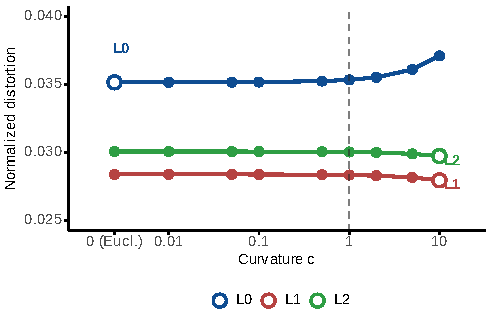
\includegraphics[width=\columnwidth]{figures/curvature_distortion.pdf}
\caption{Layer-wise curvature--distortion curves（$K=128$）。横轴为曲率 $c$（对数刻度，最左为 Euclidean 几何 $c=0$），纵轴为归一化 distortion。L0 的最低 distortion 出现在 $c=0$，而 L1/L2 的最低点位于 hyperbolic regime（$c\geq 1$），三层的 curvature preference 清晰分离。}
\label{fig:curvature-distortion}
\end{figure}

由此得到从结构异质到曲率异质的直接证据链：
\begin{equation}
\begin{gathered}
G(\mathcal{E}_0)\neq G(\mathcal{E}_1)\neq G(\mathcal{E}_2)\\[2pt]
\Downarrow\\[2pt]
\mathrm{Distortion}_0(c)\neq \mathrm{Distortion}_1(c)\neq \mathrm{Distortion}_2(c)\\[2pt]
\Downarrow\\[2pt]
c_0^{*}=0,\qquad c_1^{*},c_2^{*}\geq 1.
\end{gathered}
\end{equation}
\noindent\textbf{为什么深层偏好 hyperbolic？} 负曲率提供不同的距离扩张规律：$d$ 维双曲空间体积按
\begin{equation}
V_c(\rho)\propto \exp\!\bigl((d-1)\sqrt{c}\,\rho\bigr)
\end{equation}
近似指数增长（欧氏仅为多项式）~\cite{krioukov2010hyperbolic,gromov1987hyperbolic}；在 Poincar\'e ball 中，越接近边界双曲测地距离对位置变化越敏感（边界在双曲距离意义下位于无限远处）~\cite{nickel2017poincare,ganea2018hyperbolicnn}。因此，当某层关系需要同时保持局部接近与远距离区分时，负曲率更合适——L1/L2 恰好表现出这种需求，而 L0 不需要。

\noindent\textbf{结论。} 强制所有量化层共享曲率
\begin{equation}
c_0=c_1=c_2=c,
\end{equation}
意味着三个几何与偏好各异的 codebook 必须使用完全相同的距离扩张规律，任何单一 $c$ 都只能在两类需求间折衷——较大的 $c$ 使 L0 偏离其最优几何，较小的 $c$ 无法匹配深层 codebook 的 relational structure。允许曲率随量化层变化
\begin{equation}
c_0,\qquad c_1,\qquad c_2
\end{equation}
是更自然的建模方式。

\fbox{\parbox{0.90\columnwidth}{\textbf{核心结论：}不同 RQ stage 的 codebook geometry 与 curvature preference 均逐层异质（$G(\mathcal{E}_0)\neq G(\mathcal{E}_1)\neq G(\mathcal{E}_2)$，$c_0^{*}=0$ 而 $c_1^{*},c_2^{*}\geq1$），共享单一曲率迫使这些异质几何使用同一距离扩张规律，构成不必要的几何约束；layer-varying curvature 是更自然的建模方式。}}

最后，几何对齐不等于推荐性能：较低的 relational distortion 不能被直接解释为更高的 Recall/NDCG，其能否转化为 codeword assignment 与推荐效果的改善，需由后续 downstream experiments 独立验证~\cite{jin2024cost,topotok2026}。

\section{实验}

\subsection{复现情况：Amazon Musical\_Instruments 基线对比}

为验证生成式推荐与序列模型在目标数据集上的可比基线，我们对 Amazon 2018 Musical\_Instruments 5-core（HG-Rec 处理版，与 DIGER 同源）进行了系统复现。数据集规模为 24,772 用户 / 9,922 商品 / 206,153 交互（训练 131,837 样本，留一法 valid+test）。全部 8 组模型（BERT4Rec、GRU4Rec、SASRec、CORE、FEARec、S3Rec 六个序列推荐模型与 DIGER、DECOR 两个生成式推荐系统模型）的复现配置为 LR=0.001、batch=4096（FEARec 为 2048）、NDCG@10 早停，其中 S3Rec 采用预训练（向量化重构 50 epoch）加微调的两阶段流程。结果汇总于表~\ref{tab:repro-overall}。

\begin{table}[ht]
\centering
\small
\caption{Amazon Musical\_Instruments 5-core 复现结果对比（按 Recall@10 升序）。}
\label{tab:repro-overall}
\begin{tabular}{lcccc}
\toprule
模型 & Recall@5 & Recall@10 & NDCG@5 & NDCG@10 \\
\midrule
\multicolumn{5}{l}{\textit{序列推荐模型}} \\
BERT4Rec     & 0.0660 & 0.0824 & 0.0528 & 0.0580 \\
GRU4Rec      & 0.0713 & 0.0898 & 0.0577 & 0.0636 \\
SASRec       & 0.0790 & 0.1033 & 0.0536 & 0.0614 \\
CORE         & 0.0727 & 0.1054 & 0.0417 & 0.0523 \\
FEARec       & 0.0853 & 0.1098 & 0.0595 & 0.0674 \\
S3Rec        & 0.0834 & 0.1102 & 0.0561 & 0.0648 \\
\midrule
\multicolumn{5}{l}{\textit{生成式推荐系统模型}} \\
DIGER        & 0.0896 & 0.1127 & 0.0756 & 0.0831 \\
DECOR        & 0.0925 & 0.1157 & 0.0784 & 0.0859 \\
\bottomrule
\end{tabular}
\end{table}



复现要点如下。Recall@10 上 S3Rec（0.1102）最优，FEARec（0.1098）、CORE（0.1054）、SASRec（0.1033）、GRU4Rec（0.0898）与 BERT4Rec（0.0824）依次次之；NDCG@10 则由 FEARec（0.0674）领先，说明基于自监督/语义增强的序列模型在召回上具有竞争力。DECOR（0.1157）与 DIGER（0.1127）进一步达到约 $0.11$ 的 Recall@10 目标水平。


\begin{acks}
本文工作使用了 HG-Rec (Zhang 等, ICML 2026) 的开源复现代码与 Amazon Review 2023 公开数据集。感谢 RQ-VAE、SID 与生成式推荐领域的相关研究工作。
\end{acks}

% ===========================================================
% 参考文献
% ===========================================================
\bibliographystyle{ACM-Reference-Format}
\bibliography{per_layer_curvature_refs}

\end{document}